\chapter{الحفز العضوي الفلزي: الخطوات الأولية والدورات}\label{ch:b2:catalytic-cycles}

بضعة ملّيغرامات من ملح للبلاديوم تكفي لوصل حلقتين عطريتين في دورق
يحوي كيلوغرامات من الكواشف: فذرة الفلز نفسها تؤدي العمل آلاف
المرات، عائدة إلى حالتها الأولى بعد كل مرور. وكيفية ذلك
ترويها \omterm{def:b2:catalytic-cycles:cycle}{الدورة الحفزية}، وهي سلسلة مغلقة من بضع خطوات أولية.
وليس ثمة إلا أنواع قليلة من الخطوات، وكل منها يغيّر حالة الأكسدة، 
وعدد الإلكترونات وعدد الربائط للفلز بطريقة محددة. ومع
عدّ الإلكترونات في \cref{ch:b2:coordination-complexes}، يمكن قراءة الدورة،
والتحقق منها، والتنبؤ بها أحيانًا.

\begin{recall}
\Cref{ch:b2:coordination-complexes}: حالة الأكسدة، و$d^n$، \omterm{def:b2:coordination-complexes:electron-count}{وعدد إلكترونات التكافؤ}،
\omterm{def:b2:coordination-complexes:electron-count}{وقاعدة الثمانية عشر إلكترونًا}، \omterm{def:b2:coordination-complexes:hapticity}{والهابتية}. و\cref{ch:b2:ligand-field}: الربائط المستقبلة $\pi$ 
\omterm{def:b2:ligand-field:pi-ligands}{والتبرع العكسي}. ومجلد السنة الأولى: الحفاز، والحفز المتجانس، والخطوة الأولية،
والخطوة المحددة للسرعة، والمركب العضوي الفلزي، وعدد الأكسدة.
\end{recall}

\begin{omfigure}
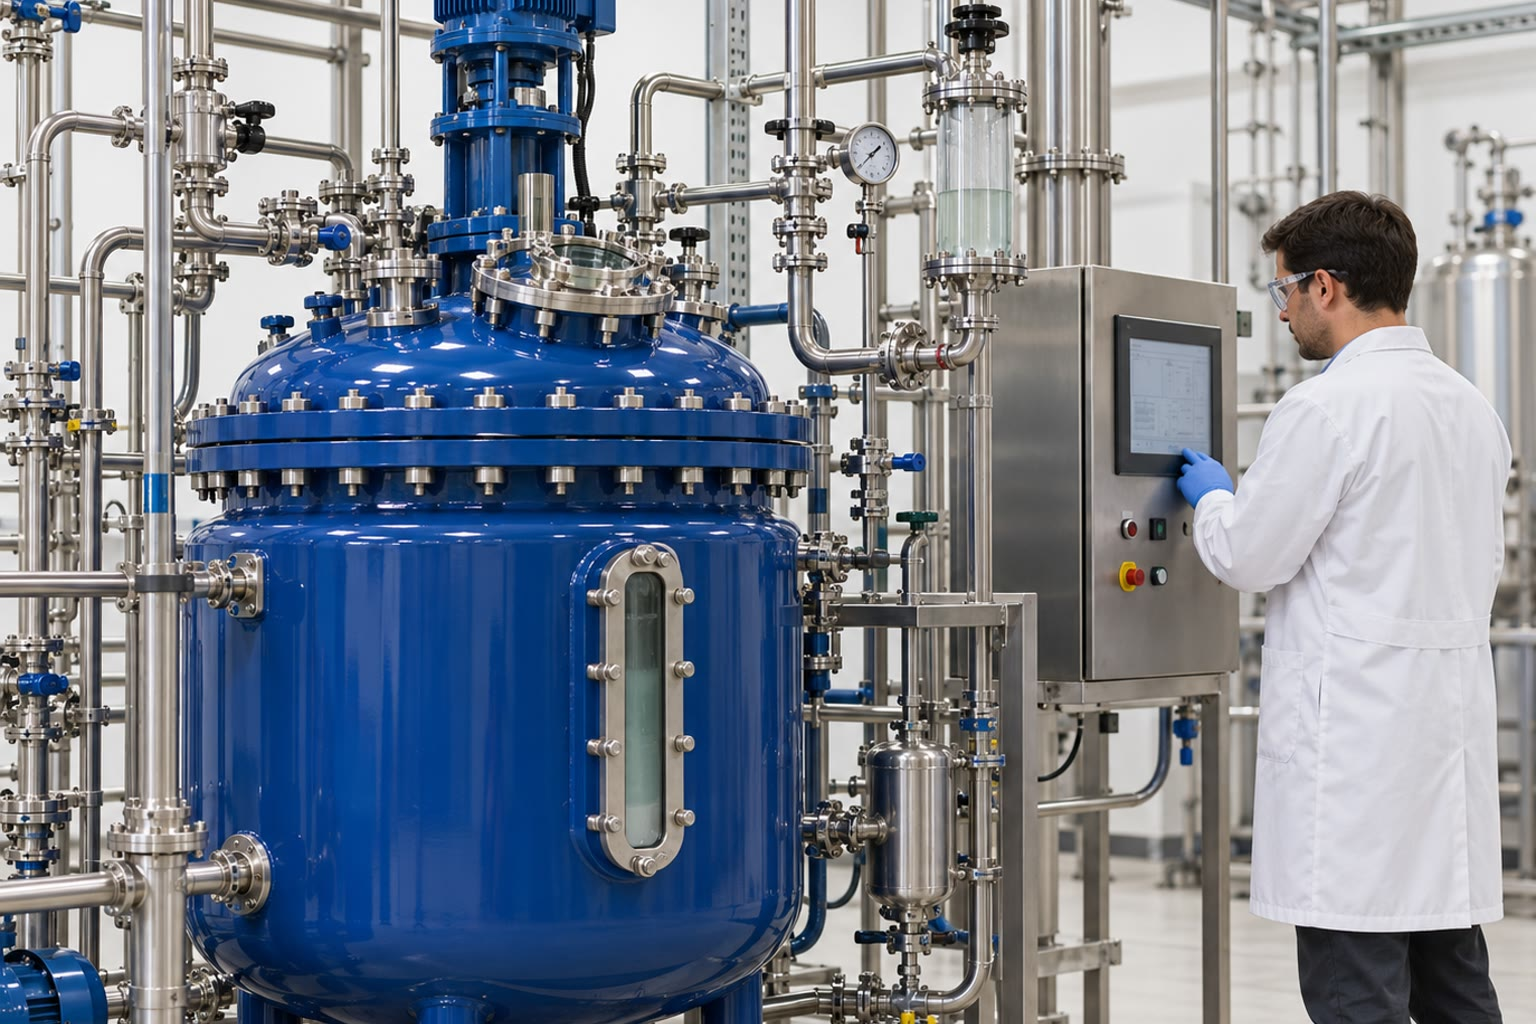
\includegraphics[width=0.62\linewidth]{images/book3/ai/b2-20-pilot-plant.jpg}

{\small وحدة تجريبية لكيمياء العمليات: مفاعل فولاذي مبطن بالزجاج، يُنقل فيه
اقتران محفَّز من حجم الدورق إلى حجم أكبر قبل الإنتاج.}
\end{omfigure}

\section{لغة المعقدات العضوية الفلزية}

تُعدّ المعقدات العضوية الفلزية كما في \cref{met:b2:coordination-complexes:electron-count}،
مع ربائط إضافية قليلة: فالهيدريد \ce{H-} وأنيون الألكيل أو الأريل \ce{R-} يعطي كل منهما
إلكترونين ويُحسب $-1$ في حالة الأكسدة؛ و\ce{CO} والفوسفينات \ce{PR3} 
والألكينات $\eta^2$ تعطي إلكترونين وتُحسب 0؛ والهاليد \ce{X-} يعطي إلكترونين ويُحسب
$-1$.

\begin{definition}[المعقدات غير المشبعة]\label{def:b2:catalytic-cycles:unsaturated}
\emph{المعقد غير المشبع تناسقيًا}\index{معقد غير مشبع تناسقيًا}
له أقل من 18 إلكترون تكافؤ (16 غالبًا) ويمكنه أن يرتبط بربيطة أخرى: فله
\emph{موقع شاغر}\index{موقع شاغر}، أي موضع في كرة تناسقه خالٍ
لاستقبال مانح لإلكترونين.
\end{definition}

المعقدات المربعة المستوية $d^8$ للروديوم(I) والإيريديوم(I) والبلاديوم(II) 
والبلاتين(II) معقدات ذات 16 إلكترونًا؛ ولمعقدات البلاديوم(0) الثنائية الفوسفين \ce{PdL2} أربعة عشر.
وهذه المعقدات هي الأنواع النشطة في معظم الدورات الحفزية.

\begin{method}[عدّ معقد عضوي فلزي]\label{met:b2:catalytic-cycles:count-organometallic}
\begin{enumerate}
  \item عدّد الربائط: الأنيونية (\ce{H-}، \ce{R-}، \ce{X-}، \ce{C5H5-}) والمتعادلة
        (\ce{CO}، \ce{PR3}، الألكينات، المذيب).
  \item حالة الأكسدة = شحنة المعقد $-$ مجموع شحنات الربائط الأنيونية.
  \item $n = g -$ حالة الأكسدة؛ والعدد = $n + 2 \times$(عدد المانحات لإلكترونين)
        $+$ 6 لكل $\eta^5$-\ce{C5H5-}.
  \item عدد التناسق = عدد مواضع الربائط المشغولة.
\end{enumerate}
\end{method}

\section{تبادل الربائط، والإضافة التأكسدية، والحذف الاختزالي}

\begin{definition}[تبادل الربائط]\label{def:b2:catalytic-cycles:ligand-exchange}
\emph{تبادل الربائط}\index{تبادل الربائط} خطوة أولية تحل فيها ربيطة أخرى محل ربيطة من
\omterm{def:b2:coordination-complexes:coordination-sphere}{كرة التناسق}؛ ولا يغيّر حالة الأكسدة
ولا، في المحصلة، عدد الإلكترونات. وتُدرس آلياته في مجلد السنة الثالثة.
\end{definition}

\begin{definition}[الإضافة التأكسدية والحذف الاختزالي]\label{def:b2:catalytic-cycles:oxidative-addition}
في \emph{الإضافة التأكسدية}\index{إضافة تأكسدية}، يُضاف جزيء A--B إلى
مركز فلزي بكسر رابطته A--B وتكوين الرابطتين M--A وM--B. 
و\emph{الحذف الاختزالي}\index{حذف اختزالي} هو الخطوة العكسية: ربيطتان
A وB، في وضع cis إحداهما بالنسبة إلى الأخرى، تتحدان في A--B وتغادران الفلز.
\end{definition}

\begin{proposition}[عدّ الإضافة التأكسدية]\label{prop:b2:catalytic-cycles:oa}
ترفع \omterm{def:b2:catalytic-cycles:oxidative-addition}{الإضافة التأكسدية} حالة أكسدة الفلز بمقدار 2، وعدد إلكترونات تكافئه
بمقدار 2 وعدد تناسقه بمقدار 2؛ ويخفض \omterm{def:b2:catalytic-cycles:oxidative-addition}{الحذف الاختزالي} كلًّا منها بمقدار 2.
\end{proposition}

\begin{proof}
تُحسب A وB أنيونات (\ce{H-}، \ce{R-}، \ce{X-}) بعد ارتباطهما: فالربيطتان الأنيونيتان
الجديدتان ترفعان حالة الأكسدة بمقدار 2 وتخفضان $n$ بمقدار 2؛ وتقدمان زوجين، أي $+4$
إلكترونات؛ فيتغير العدد بمقدار $-2 + 4 = +2$. ويُشغل موضعان جديدان. 
والخطوة العكسية تعكس كل تغيير.
\end{proof}

\begin{example}[معقد فاسكا]\label{ex:b2:catalytic-cycles:vaska}
\ce{[IrCl(CO)(PPh3)2]}، مربع مستوٍ: إيريديوم(I)، $d^8$، 16 إلكترونًا، رباعي التناسق.
ويضيف ثنائي الهيدروجين: \ce{[IrH2Cl(CO)(PPh3)2]}، إيريديوم(III)، $d^6$، 18 إلكترونًا، ثماني الأوجه،
والهيدريدان في وضع cis.
\end{example}

\section{الإدخال، والحذف، والتبادل الفلزي}

\begin{definition}[الإدخال وحذف الهيدريد $\beta$]\label{def:b2:catalytic-cycles:insertion}
في \emph{الإدخال الهجري}\index{إدخال هجري}، تُدخَل ربيطة غير مشبعة
(ألكين، \ce{CO}) مرتبطة بالفلز في رابطة M--H أو M--C مجاورة في وضع cis: فيعطي \ce{M-H} 
وألكين ألكيلًا \ce{M-CH2-CH2-H}؛ ويعطي \ce{M-R} و\ce{CO} أسيلًا \ce{M-C(=O)R}.
و\emph{حذف الهيدريد $\beta$}\index{حذف الهيدريد بيتا@حذف الهيدريد $\beta$}
هو عكس إدخال الألكين: ينتقل هيدروجين على الكربون $\beta$ بالنسبة إلى
الفلز إلى الفلز، فيتحرر ألكين.
\end{definition}

\begin{proposition}[عدّ الإدخال]\label{prop:b2:catalytic-cycles:insertion}
يحافظ \omterm{def:b2:catalytic-cycles:insertion}{الإدخال الهجري} على حالة الأكسدة ويخفض عدد الإلكترونات بمقدار 2
(إذ يتحرر موضع ربيطة)؛ ويرفع حذف الهيدريد $\beta$ العدد بمقدار 2.
\end{proposition}

\begin{proof}
قبله: \ce{H-} (أو \ce{R-}، الأنيوني) والألكين (المتعادل)، ربيطتان، أربعة إلكترونات.
وبعده: ألكيل واحد (أنيوني)، إلكترونان. والشحنة الأنيونية لم تتغير: حالة
الأكسدة نفسها؛ وقد فُقد إلكترونان وموضع واحد.
\end{proof}

\begin{proposition}[شروط حذف الهيدريد $\beta$]\label{prop:b2:catalytic-cycles:beta-h}
لا يخضع ألكيل الفلز لحذف الهيدريد $\beta$ إلا إذا حمل الألكيل هيدروجينًا على
كربونه $\beta$ وكان للفلز \omterm{def:b2:catalytic-cycles:unsaturated}{موقع شاغر} في وضع cis بالنسبة إلى الألكيل.
\end{proposition}

\begin{proof}[تعليل]
تمر الخطوة بترتيب رباعي \babelsublr{M--C$_\alpha$--C$_\beta$--H} يبلغ فيه
الهيدروجين الفلز: فهي تحتاج إلى ذلك الهيدروجين، وإلى موضع فارغ مجاور للألكيل
لاستقباله. ومجموعات الميثيل والبنزيل والنيوبنتيل والأريل، التي ليس لها هيدروجين $\beta$
قادر على بلوغ الفلز، مستقرة تجاهها.
\end{proof}

\begin{definition}[التبادل الفلزي]\label{def:b2:catalytic-cycles:transmetalation}
\emph{التبادل الفلزي}\index{تبادل فلزي} ينقل مجموعة عضوية من فلز
(أو شبه فلز: البور، الزنك، القصدير) إلى آخر، مقابل هاليد في العادة.
\end{definition}

\begin{omfigure}
\begin{tikzpicture}[font=\small, >={Stealth}]
  \tikzset{omstepar/.style={->, thick}}
  \foreach \y/\l/\r/\top/\bot/\rev/\dum in {
      0/{$\mathrm{L}_n\mathrm{M}$}/{$\mathrm{L}_n\mathrm{M(A)(B)}$}/{+ A--B}/{\foreignlanguage{arabic}{إضافة تأكسدية}}/{\foreignlanguage{arabic}{حذف اختزالي}}/{},
      -1.5/{$\mathrm{L}_n\mathrm{M(H)(CH_2{=}CH_2)}$}/{$\mathrm{L}_n\mathrm{M{-}CH_2CH_3}$}/{}/{\foreignlanguage{arabic}{إدخال هجري}}/{\foreignlanguage{arabic}{حذف الهيدريد $\beta$}}/{},
      -3.0/{$\mathrm{L}_n\mathrm{M(X)(R)}$}/{$\mathrm{L}_n\mathrm{M(R)(R')}$}/{+ R$'$--[B], $-$ X--[B]}/{\foreignlanguage{arabic}{تبادل فلزي}}/{}/{},
      -4.5/{$\mathrm{L}_n\mathrm{M(X)}$}/{$\mathrm{L}_n\mathrm{M(X)(L')}$}/{+ L$'$}/{\foreignlanguage{arabic}{تبادل ربيطة أو ارتباطها}}/{}/{}} {
    \node[cyclenode, anchor=east] (l) at (0,\y) {\l};
    \node[cyclenode, anchor=west] (r) at (5.2,\y) {\r};
    \draw[omstepar] ($(l.east)+(0.1,0.08)$) -- ($(r.west)+(-0.1,0.08)$) node[midway, above, font=\scriptsize] {\top};
    \node[font=\scriptsize, anchor=north] at (2.6,\y-0.02) {\bot};
    \node[font=\scriptsize, black!55, anchor=west] at (5.2,\y-0.5) {\rev};
  }
\end{tikzpicture}

{\small الخطوات الأولية للحفز العضوي الفلزي. \omterm{def:b2:catalytic-cycles:oxidative-addition}{الإضافة التأكسدية}: حالة
الأكسدة والعدد وعدد التناسق $+2$؛ \omterm{def:b2:catalytic-cycles:oxidative-addition}{والحذف الاختزالي}: $-2$. \omterm{def:b2:catalytic-cycles:insertion}{والإدخال
الهجري}: العدد $-2$، وحالة الأكسدة دون تغيير؛ وحذف الهيدريد $\beta$: عكسه.
\omterm{def:b2:catalytic-cycles:transmetalation}{والتبادل الفلزي}: تنتقل مجموعة عضوية إلى الفلز من البور أو الزنك أو القصدير.}
\end{omfigure}

\section{قراءة دورة حفزية}

\begin{definition}[الدورة الحفزية]\label{def:b2:catalytic-cycles:cycle}
\emph{الدورة الحفزية}\index{دورة حفزية} سلسلة مغلقة من الخطوات الأولية
تستهلك الكواشف، وتحرر النواتج وتجدد معقدها الأول. 
والمركب المضاف إلى التفاعل، الذي يتحول إلى المعقد الأول في الدورة، هو
\emph{طليعة الحفاز}\index{طليعة الحفاز}. و\emph{عدد الدوران}\index{عدد الدوران}
(TON) هو كمية الناتج المتكوّن لكل كمية من الحفاز؛ و\emph{تردد
الدوران}\index{تردد الدوران} (TOF) هو عدد الدوران في وحدة الزمن.
\end{definition}

\begin{proposition}[المعادلة الإجمالية]\label{prop:b2:catalytic-cycles:cycle-sum}
مجموع خطوات \omterm{def:b2:catalytic-cycles:cycle}{الدورة الحفزية} هو معادلة التفاعل المحفَّز:
فكل معقد فلزي يظهر مرة ناتجًا ومرة متفاعلًا، فيُختزل.
\end{proposition}

\begin{proof}
لما كانت الدورة مغلقة، فكل مركب وسيط تكوّنه خطوة وتستهلكه الخطوة التالية؛
وبجمع الخطوات، تظهر هذه الأنواع في الطرفين فتُختزل. ويبقى
ما يدخل من الخارج (الكواشف) وما يخرج (النواتج).
\end{proof}

\begin{method}[قراءة دورة]\label{met:b2:catalytic-cycles:read-cycle}
\begin{enumerate}
  \item لكل معقد، احسب حالة الأكسدة وعدد الإلكترونات 
        وعدد التناسق.
  \item سمِّ كل خطوة من التغيرات ($+2/+2/+2$: \omterm{def:b2:catalytic-cycles:oxidative-addition}{إضافة تأكسدية}؛ العدد $-2$ عند
        حالة أكسدة ثابتة: إدخال؛ وهكذا).
  \item تحقق من أن أي معقد لا يتجاوز 18 إلكترونًا وأن كل خطوة تحتاج إلى \omterm{def:b2:catalytic-cycles:unsaturated}{موقع شاغر}
        تبدأ من معقد غير مشبع.
  \item اجمع الخطوات: يجب أن يكون المجموع هو المعادلة الإجمالية.
\end{enumerate}
\end{method}

\begin{omfigure}
\begin{tikzpicture}[font=\small, >={Stealth}]
  \node[cyclenode] (n1) at (90:2.3) {\ce{[RhCl(PPh3)2]}\\ Rh(I), 14 e};
  \node[cyclenode] (n2) at (0:3.4) {\ce{[RhH2Cl(PPh3)2]}\\ Rh(III), 16 e};
  \node[cyclenode] (n3) at (270:2.3) {\ce{[RhH2Cl(PPh3)2(RCH=CH2)]}\\ Rh(III), 18 e};
  \node[cyclenode] (n4) at (180:3.4) {\ce{[RhH(CH2CH2R)Cl(PPh3)2]}\\ Rh(III), 16 e};
  \draw[cyclearc] (n1) to[bend left=20] node[cyclelabel, below left] {\foreignlanguage{arabic}{إضافة}\\ \foreignlanguage{arabic}{تأكسدية}} (n2);
  \draw[cyclearc] (n2) to[bend left=20] node[cyclelabel, left=12pt] {\foreignlanguage{arabic}{ارتباط}\\ \foreignlanguage{arabic}{الألكين}} (n3);
  \draw[cyclearc] (n3) to[bend left=20] node[cyclelabel, above right] {\foreignlanguage{arabic}{إدخال}\\ \foreignlanguage{arabic}{هجري}} (n4);
  \draw[cyclearc] (n4) to[bend left=20] node[cyclelabel, below right] {\foreignlanguage{arabic}{حذف}\\ \foreignlanguage{arabic}{اختزالي}} (n1);
  \draw[cyclein] (4.6,2.3) node[right] {\ce{H2}} -- (2.6,1.75);
  \draw[cyclein] (4.6,-2.3) node[right] {ألكين} -- (2.6,-1.75);
  \draw[cycleout] (-2.6,1.75) -- (-4.6,2.3) node[left] {ألكان};
  \node[font=\scriptsize, align=center, black!60] at (0,-0.05) {\foreignlanguage{arabic}{طليعة الحفاز}\\ \ce{[RhCl(PPh3)3]}\\ \foreignlanguage{arabic}{تفقد \ce{PPh3} واحدًا}};
\end{tikzpicture}

{\small هدرجة ألكين بحفاز ويلكنسون، مبسّطة (أُغفلت تبادلات الفوسفين
والمذيب). مجموع الخطوات الأربع هو $\ce{RCH=CH2 + H2 -> RCH2CH3}$؛ 
ومعقدات الروديوم تُختزل.}
\end{omfigure}

\begin{omfigure}
\begin{tikzpicture}[font=\small, >={Stealth}]
  \node[cyclenode] (s1) at (90:2.3) {\ce{PdL2}\\ Pd(0), 14 e};
  \node[cyclenode] (s2) at (0:3.4) {\ce{[ArPd(Br)L2]}\\ Pd(II), 16 e};
  \node[cyclenode] (s3) at (270:2.3) {$[\mathrm{ArPd(Ar')L_2}]$\\ Pd(II), 16 e};
  \draw[cyclearc] (s1) to[bend left=25] node[cyclelabel, below left] {\foreignlanguage{arabic}{إضافة}\\ \foreignlanguage{arabic}{تأكسدية}} (s2);
  \draw[cyclearc] (s2) to[bend left=25] node[cyclelabel, above left] {\foreignlanguage{arabic}{تبادل فلزي}} (s3);
  \draw[cyclearc] (s3) to[bend left=35] node[cyclelabel, right] {\foreignlanguage{arabic}{حذف}\\ \foreignlanguage{arabic}{اختزالي}} (s1);
  \draw[cyclein] (4.8,2.2) node[right] {\ce{Ar-Br}} -- (2.6,1.6);
  \draw[cyclein] (5.4,-0.9) node[right, align=left] {$\mathrm{Ar'B(OH)_2}$\\ \foreignlanguage{arabic}{+ قاعدة}} -- (3.3,-1.2);
  \draw[cycleout] (2.3,-2.0) -- (4.4,-2.9) node[right] {\ce{Br-}، \ce{B(OH)3}};
  \draw[cycleout] (-1.75,-0.4) -- (-4.2,-0.4) node[left] {$\mathrm{Ar{-}Ar'}$};
\end{tikzpicture}

{\small اقتران سوزوكي، مبسّطًا. يضيف البلاديوم(0) بروميد الأريل؛ وتحوّل القاعدة
حمض البورونيك إلى بورات، تنقل مجموعتها الأريلية إلى البلاديوم؛ ثم تُحذف
مجموعتا الأريل، وهما في وضع cis، على هيئة ثنائي الأريل، فيتجدد البلاديوم(0).}
\end{omfigure}

في تفاعل هيك، يرتبط معقد الأريل--بلاديوم المتكوّن \omterm{def:b2:catalytic-cycles:oxidative-addition}{بالإضافة التأكسدية} بألكين
بدلًا من بورات؛ ويضع \omterm{def:b2:catalytic-cycles:insertion}{الإدخال الهجري} الأريل على الألكين، ثم يحرر
حذف الهيدريد $\beta$ الألكين المستبدَل (المتماكب trans عادة)
وهيدريد بلاديوم، تنزع منه قاعدة \ce{HBr} فيتجدد البلاديوم(0).

والهيدروفورميلة، أي إضافة \ce{H2} و\ce{CO} عبر ألكين لإعطاء ألدهيد،
تجري على هيدريدات الكوبالت أو الروديوم بإدخال الألكين، ثم إدخال \ce{CO}
في الرابطة فلز--ألكيل، ثم \omterm{def:b2:catalytic-cycles:oxidative-addition}{الإضافة التأكسدية} للهيدروجين \ce{H2} \omterm{def:b2:catalytic-cycles:oxidative-addition}{والحذف الاختزالي}
للألدهيد. واتجاه الإدخال الأول يحدد الناتج: فالفلز على الكربون
الطرفي يعطي الألدهيد الخطي، وعلى الكربون الداخلي الألدهيد المتفرع؛ 
والفوسفينات الضخمة تفضّل الناتج الخطي.

\begin{history}[الاقتران المتصالب]
\begin{minipage}[t]{0.36\linewidth}
\vspace{0pt}
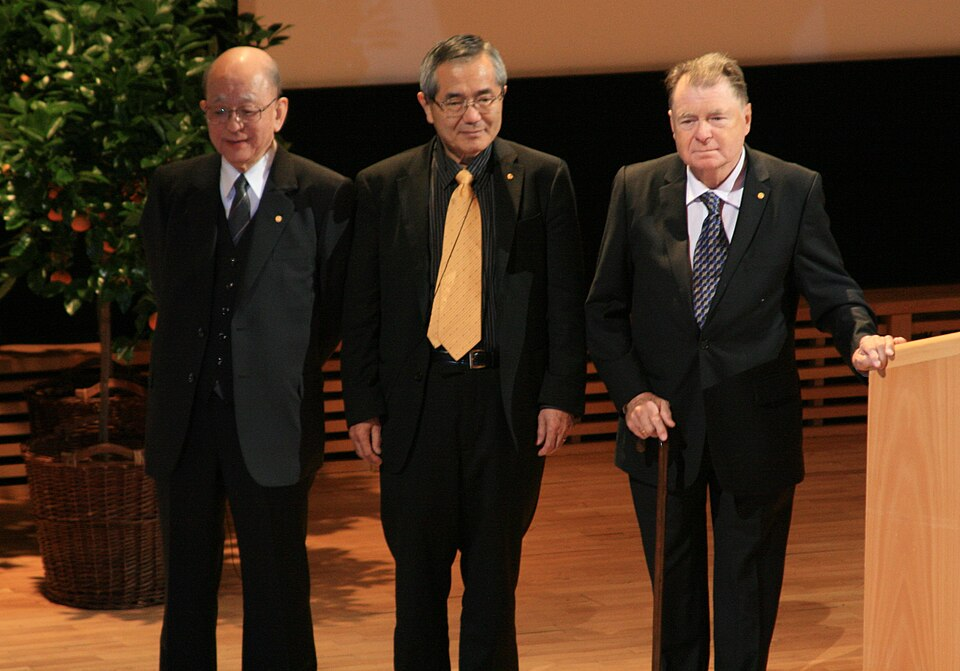
\includegraphics[width=\linewidth]{images/book3/nobel-2010.jpg}
\end{minipage}\hfill
\begin{minipage}[t]{0.6\linewidth}
\vspace{0pt}
اقترانات أهاليد الأريل والفينيل المحفَّزة بالبلاديوم مع الألكينات (ريتشارد هيك، منذ
1968)، ومع الكواشف العضوية للزنك (إي-إيتشي نيغيشي، 1977) ومع مركبات البور العضوية
(أكيرا سوزوكي، 1979) جعلت وصل هيكلين كربونيين أمرًا معتادًا؛ وهي اليوم من
أكثر التفاعلات استعمالًا في صنع الأدوية والمواد. ومُنحت جائزة نوبل في
الكيمياء للثلاثة سنة 2010. (صورة: سوزوكي ونيغيشي وهيك، من اليسار
إلى اليمين، 2010؛ بلودآيس، CC~BY-SA~4.0، ويكيميديا كومنز.)
\end{minipage}
\end{history}

\begin{proposition}[الدوران]\label{prop:b2:catalytic-cycles:tof}
إذا كانت $n_P$ كمية الناتج المتكوّن في زمن $t$ بكمية $n_{\text{حفاز}}$ من الحفاز، فإن
$\mathrm{TON} = n_P/n_{\text{حفاز}}$ ويكون متوسط \omterm{def:b2:catalytic-cycles:cycle}{تردد الدوران} $\mathrm{TOF} =
\mathrm{TON}/t$.
\end{proposition}

\begin{proof}
كل دورة تصنع جزيء ناتج واحدًا لكل ذرة فلز؛ وعدد الدورات التي تتمها
كل ذرة في المتوسط هو $n_P/n_{\text{حفاز}}$، ومعدل الدوران هو ذلك العدد في وحدة
الزمن.
\end{proof}

\begin{safety}{\ghs[5mm]{GHS05}\,\ghs[5mm]{GHS07}\,\ghs[5mm]{GHS09}}
إيثانوات البلاديوم(II) أكّالة للعينين وسامة للأحياء المائية؛
والثلاثي فينيل الفوسفين ضار ومحسِّس. وتوزن تحت ساحبة أبخرة، 
وتُجمع بقايا البلاديوم لاستعادتها، ولا تُسكب أبدًا في المجرى.
% ledger: ghs:Pd-acetate, ghs:PPh3, ghs:phenylboronic-acid, ghs:4-bromotoluene
\end{safety}

\section{تمارين}

\begin{exercise}[$\star$]\label{exo:b2:catalytic-cycles:1}
أعطِ حالة الأكسدة و$d^n$ وعدد الإلكترونات لمعقد فاسكا
\ce{[IrCl(CO)(PPh3)2]} قبل إضافته \ce{H2} وبعدها.
\end{exercise}

\begin{exercise}[$\star$]\label{exo:b2:catalytic-cycles:2}
سمِّ الخطوة: \ce{[PtCl2(CH3)2(PR3)2] -> [PtCl2(PR3)2] + C2H6}؛ \ce{[Pd(Ph)Br(PR3)2] +
CH2=CH2 -> [Pd(CH2CH2Ph)Br(PR3)] + PR3}.
\end{exercise}

\begin{exercise}[$\star$]\label{exo:b2:catalytic-cycles:3}
يستعمل تفاعل \qty{0.020}{mmol} من الحفاز ويعطي \qty{15.0}{mmol} من الناتج في
\qty{3.0}{h}. احسب TON ومتوسط TOF.
\end{exercise}

\begin{exercise}[$\star$]\label{exo:b2:catalytic-cycles:4}
اجمع خطوات دورة سوزوكي الثلاث وتحقق من أن البلاديوم يُختزل.
\end{exercise}

\begin{exercise}[$\star\star$]\label{exo:b2:catalytic-cycles:5}
أي معقدات ألكيل البلاديوم هذه يمكن أن تخضع لحذف الهيدريد $\beta$:
\ce{Pd-CH3}، \ce{Pd-CH2CH3}، \ce{Pd-CH2C(CH3)3}، \ce{Pd-CH2Ph}، \ce{Pd-CH(CH3)2}؟
\end{exercise}

\begin{exercise}[$\star\star$]\label{exo:b2:catalytic-cycles:6}
تنبأ بناتج تفاعل هيك بين اليودوبنزين وبروبينوات الميثيل، وبهندسته.
\end{exercise}

\begin{exercise}[$\star\star$]\label{exo:b2:catalytic-cycles:7}
اكتب الألدهيدين الخطي والمتفرع الناتجين من هيدروفورميلة البروبين، 
وفسّر أي إدخال يؤدي إلى كل منهما.
\end{exercise}

\begin{exercise}[$\star\star$]\label{exo:b2:catalytic-cycles:8}
لماذا لا يستطيع \ce{[RhCl(PPh3)3]} إضافة \ce{H2} إلا بعد فقد فوسفين، بينما
يضيفه \ce{[RhCl(PPh3)2]} فورًا؟
\end{exercise}

\begin{exercise}[$\star\star$]\label{exo:b2:catalytic-cycles:9}
في اقتران سوزوكي، لماذا تلزم قاعدة، وماذا تفعل بحمض البورونيك؟
\end{exercise}

\begin{exercise}[$\star\star\star$]\label{exo:b2:catalytic-cycles:10}
دورة مقترحة لهدرجة ألكين على معقد $d^8$ \ce{ML3X} (16 إلكترونًا)
تبدأ بارتباط الألكين لإعطاء معقد ذي 20 إلكترونًا، ثم \omterm{def:b2:catalytic-cycles:oxidative-addition}{الإضافة التأكسدية}
للهيدروجين \ce{H2}. أوجد الخطأ وصحّح الترتيب.
\end{exercise}

\begin{exercise}[$\star\star\star$]\label{exo:b2:catalytic-cycles:11}
تزداد كمية ناتج تفاعل محفَّز وفق $n_P(t) = n_{\max}(1 - \mathrm e^{-t/\tau})$
مع $n_{\max} = \qty{10.0}{mmol}$، و$\tau = \qty{40}{min}$ و\qty{0.010}{mmol} من الحفاز
(معطيات التمرين). احسب TOF الابتدائي وTON النهائي.
\end{exercise}

\begin{exercise}[$\star\star\star$]\label{exo:b2:catalytic-cycles:12}
اقترح اقترانًا متصالبًا لتحضير 4-ميثوكسي ثنائي الفينيل، باختيار الهاليد وحمض
البورونيك، واكتب الدورة.
\end{exercise}

\section{مسألة: قراءة دورة سوزوكي}

\begin{problem}[{مسألة نهاية الأسبوع --- طليعة الحفاز والبلاديوم(0) النشط، 
والإضافة التأكسدية والتبادل الفلزي والحذف الاختزالي في اقتران سوزوكي، 
والمردود وعدد الدوران، والتفاعلات الجانبية}]
\label{pb:b2:catalytic-cycles:1}
التجربة (معطيات التمرين): \qty{10.0}{mmol} من 4-بروموتولوين، و\qty{12.0}{mmol} من
حمض الفينيل بورونيك، و\qty{20}{mmol} من كربونات البوتاسيوم، و\qty{0.050}{mmol} من إيثانوات
البلاديوم(II) و\qty{0.10}{mmol} من الثلاثي فينيل الفوسفين في خليط من التولوين والإيثانول 
والماء، مسخّن تحت النيتروجين؛ والناتج المعزول: \qty{1.51}{g} من 4-ميثيل ثنائي الفينيل. الكتل
المولية (\unit{g/mol}): 4-بروموتولوين 171.04، وحمض الفينيل بورونيك 121.93، و4-ميثيل ثنائي الفينيل
168.24، وإيثانوات البلاديوم(II) 224.51.
% ledger: aw:C, aw:H, aw:Br, aw:B, aw:O, aw:Pd

\medskip
\noindent\textbf{الجزء الأول --- الحفاز.}
\begin{enumerate}
  \item أعطِ حالة الأكسدة و$d^n$ للبلاديوم في إيثانوات البلاديوم(II).
  \item يُختزل في الدورق إلى \ce{Pd(PPh3)2}. أعطِ حالة أكسدته و$d^n$ 
        وعدد إلكتروناته.
  \item لماذا يكون ذلك \omterm{def:b2:catalytic-cycles:unsaturated}{المعقد غير مشبع تناسقيًا}؟
  \item لماذا يُجرى التفاعل تحت النيتروجين؟
  \item ما دور الفائض من الثلاثي فينيل الفوسفين؟
  \item هل إيثانوات البلاديوم(II) هي الحفاز أم \omterm{def:b2:catalytic-cycles:cycle}{طليعة الحفاز}؟
\end{enumerate}

\medskip
\noindent\textbf{الجزء الثاني --- الخطوات.}
\begin{enumerate}[resume]
  \item اكتب \omterm{def:b2:catalytic-cycles:oxidative-addition}{الإضافة التأكسدية} للمركب 4-بروموتولوين وعُدّ إلكترونات الناتج.
  \item ماذا تفعل الكربونات بحمض الفينيل بورونيك؟
  \item اكتب \omterm{def:b2:catalytic-cycles:transmetalation}{التبادل الفلزي}.
  \item لماذا يجب أن تكون مجموعتا الأريل في وضع cis قبل الخطوة التالية؟
  \item اكتب \omterm{def:b2:catalytic-cycles:oxidative-addition}{الحذف الاختزالي} وعُدّ إلكترونات نوع البلاديوم المتكوّن.
  \item اجمع الخطوات الثلاث.
\end{enumerate}

\medskip
\noindent\textbf{الجزء الثالث --- المردود والدوران.}
\begin{enumerate}[resume]
  \item أي الكواشف محدد؟
  \item احسب كمية الناتج المعزول.
  \item احسب المردود.
  \item احسب حمولة الحفاز بالنسبة المئوية المولية (mol~\%) بالنسبة إلى البروميد.
  \item احسب \omterm{def:b2:catalytic-cycles:cycle}{عدد الدوران} للبلاديوم.
  \item استغرقت التجربة \qty{4.0}{h}. احسب متوسط \omterm{def:b2:catalytic-cycles:cycle}{تردد الدوران} في الساعة.
\end{enumerate}

\medskip
\noindent\textbf{الجزء الرابع --- التفاعلات الجانبية.}
\begin{enumerate}[resume]
  \item يوجد قليل من ثنائي الفينيل \ce{Ph-Ph}. اقترح كيف يتكوّن.
  \item لماذا لا يمكن هنا أي حذف للهيدريد $\beta$؟
  \item يتفاعل كلوريد الأريل أبطأ بكثير من البروميد. أي خطوة تتأثر؟
  \item ماذا يحل بالبلاديوم في نهاية التفاعل، ولماذا يُستعاد؟
  \item لماذا يُستعمل فائض صغير من حمض البورونيك؟
  \item اذكر \omterm{def:b2:catalytic-cycles:cycle}{عدد الدوران} للبلاديوم في هذه التجربة.
\end{enumerate}
\end{problem}
